\section{Theorie}
\label{sec:Theorie}
In diesem Versuch werden selbst keine quantenmechanischen Systeme behandelt. Es lassen sich allerdings durch die Betrachtung von akustischen Phänomenen Analogien zu quantenmechanischen Systemen finden, die insbesondere auf ähnlichen mathematischen Strukturen der theoretischen Lösung der Probleme basieren. Auf Unterschiede in den Systemen wird stets hingewiesen, dennoch sind die Analogien ausreichend, um durch die Betrachtung der in diesem Versuch untersuchten Modelle einige Grundlagen der Quantenmechanik kennenzulernen. Im Folgenden sollen zwei konkrete physikalische Systeme untersucht werden, jeweils in einer klassischen und in einer quantenmechanischen Version, um danach die Zusammenhänge zu diskutieren.\\
Dieses Kapitel basiert zum Teil auf den Ausführungen aus Referenz \cite{anderesProtokoll}, welche zu einem auführlicheren Studium der theoretischen Grundlagen herangezogen werden kann.

\subsection{Eindimensionale Systeme}
\label{subsec:eindimsyst}
\subsubsection{Der eindimensionale Resonator}
Betrachtet werden soll ein Rohr mit verschlossenen Enden. Bei perfekter Reflexion einer einfallenden Welle bildet sich eine stehende Welle mit Geschwindigkeitsknoten und Druckbäuchen an den Enden aus. Die Bedingung an Wellenlänge bzw. Frequenz und Schallgeschwindigkeit lautet
\begin{equation}
  \lambda_n = \frac{c}{f_n} = \frac{2L}{n}\,.
  \label{eqn:stehendeWelle}
\end{equation}
Dabei bezeichnet $\lambda_n$ die Wellenlänge der $n$-ten Mode mit $n$ Bäuchen der Geschwindigkeit, $f_n$ die Frequenz dieser Mode, $c$ die Schallgeschwindigkeit und $n$ ist eine natürliche Zahl, 0 ausgenommen.
Diese Beziehung lässt sich aus der Forderung nach der Beschaffenheit der Welle in Bezug auf ihre Knoten und Bäuche, aus der Interferenz von einlaufender und reflektierter Welle oder der Lösung der Wellengleichung mit entsprechenden Randbedingungen ableiten. Diese lautet
\begin{equation}
  \frac{\partial^2 p(\vec{r},t)}{\partial t^2} = \frac{1}{\rho \kappa} \Laplace p(\vec{r},t)\,,
  \label{eqn:wellengleichung}
\end{equation}
wobei $p$ den Druck, $t$ die Zeit, $\rho$ die Dichte, $\kappa$ die Kompressibilität des Mediums und $\Laplace$ den Laplace-Operator bezeichnet, der hier eindimensional zu verstehen ist. Die Schallgeschwindigkeit ist durch $c^2 = \frac{1}{\rho \kappa}$ bestimmt.\\
Die Lösung dieser Gleichung unter den gegebenen Bedingungen für den Druck ist
\begin{equation}
  p(x,t) = p_\text{m} \cos\left(\frac{n \pi x}{L}\right) \cos(\omega t)\,.
  \label{eqn:stehendeWelle2}
\end{equation}
Mithilfe der Relation $\omega = ck$ mit der Kreisfrequenz $\omega = 2 \pi f$ und der Wellenzahl $k = 2 \pi / \lambda$ folgt
\begin{equation}
  \omega(k) = \frac{\pi c}{L} n\,.
  \label{eqn:dispersionKlassisch}
\end{equation}
In Abbildung \ref{fig:stehendeWelle} ist eine stehende Welle in einem Rohr für drei Zeiten zu sehen. An den Orten ohne Luftbewegung können die Teilchen als ortsfest angesehen werden. Die Pfeile drücken die Richtung aus, in die sich die Teilchen im Rohr aufgrund der Schallwelle bewegen. Es sei jedoch darauf hingewiesen, dass die Amplitude der Schwingung im Teilchenort viel kleiner gegenüber der Ausdehnung eines üblichen Rohrs ist und somit eher die Druckschwankung mit der Erscheinung der stehenden Welle assoziiert wird. Die fett gezeichneten Linien drücken gerade diese Druckschwankung aus. Orte ohne Luftbewegung und Orte ohne Druckschwankung sind nicht identisch, sondern um eine Viertel Wellenlänge verschoben.

\begin{figure}[H]
\centering
\subcaptionbox{Skizze der Luftbewegung und der Druckschwankung bei einer stehenden Welle \cite{stehendeWelle}.}%
  [.4\linewidth]{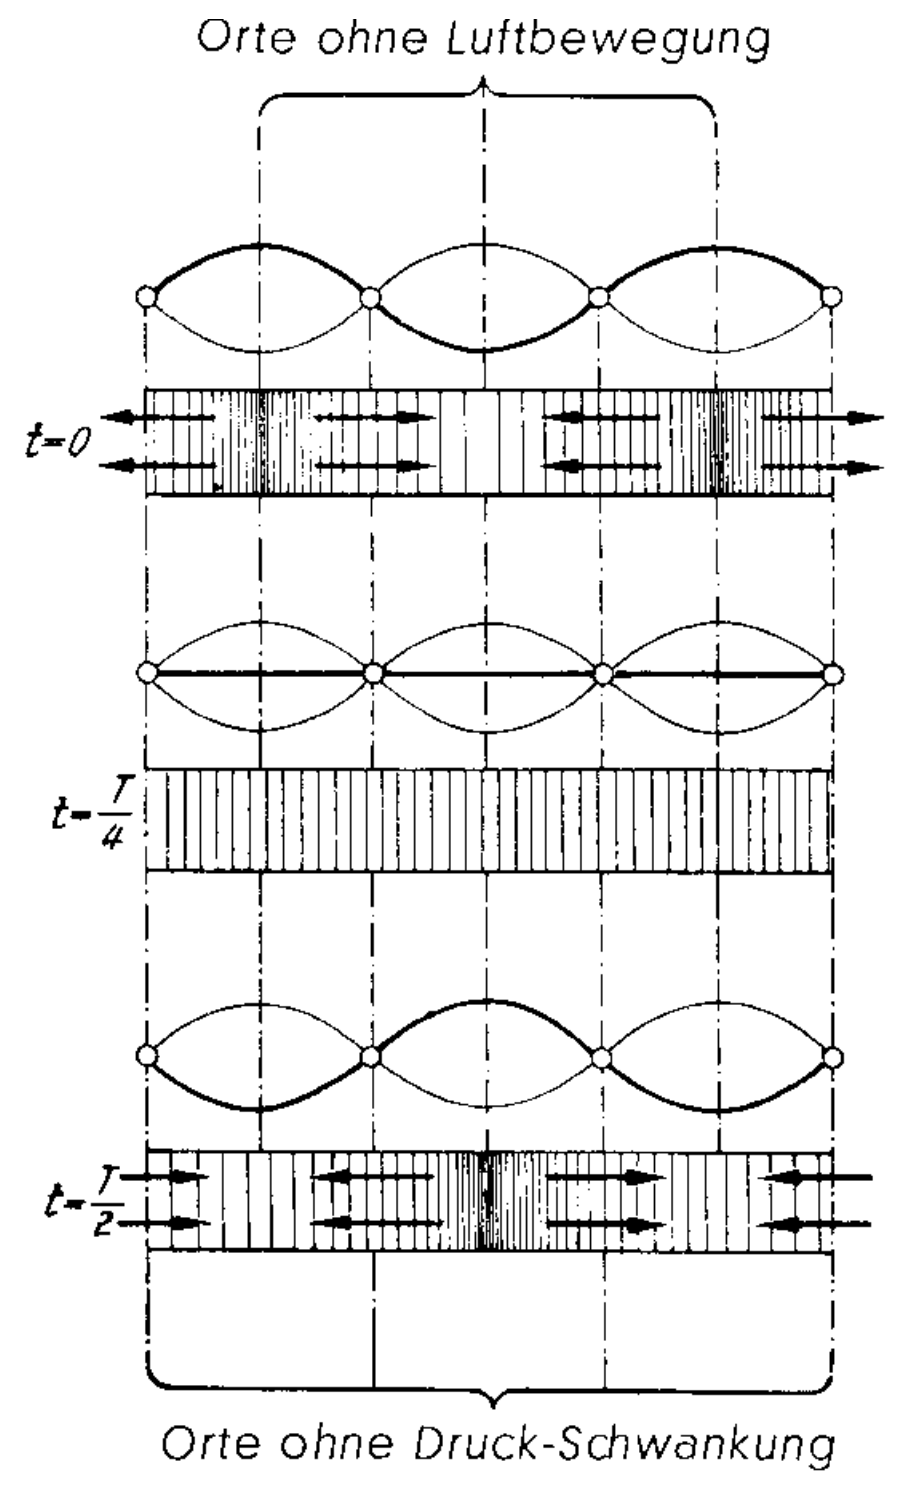
\includegraphics[width=.4\linewidth]{data/stehendeWelle.png}}
  \label{fig:stehendeWelle}
\,\,\,\,\,\,\,\,\,\,\,\,
\subcaptionbox{Schematische Darstellung der ersten vier Wellenfunktionen im unendlich hohen Potenzialtopf \cite{kasten}.}
  [.4\linewidth]{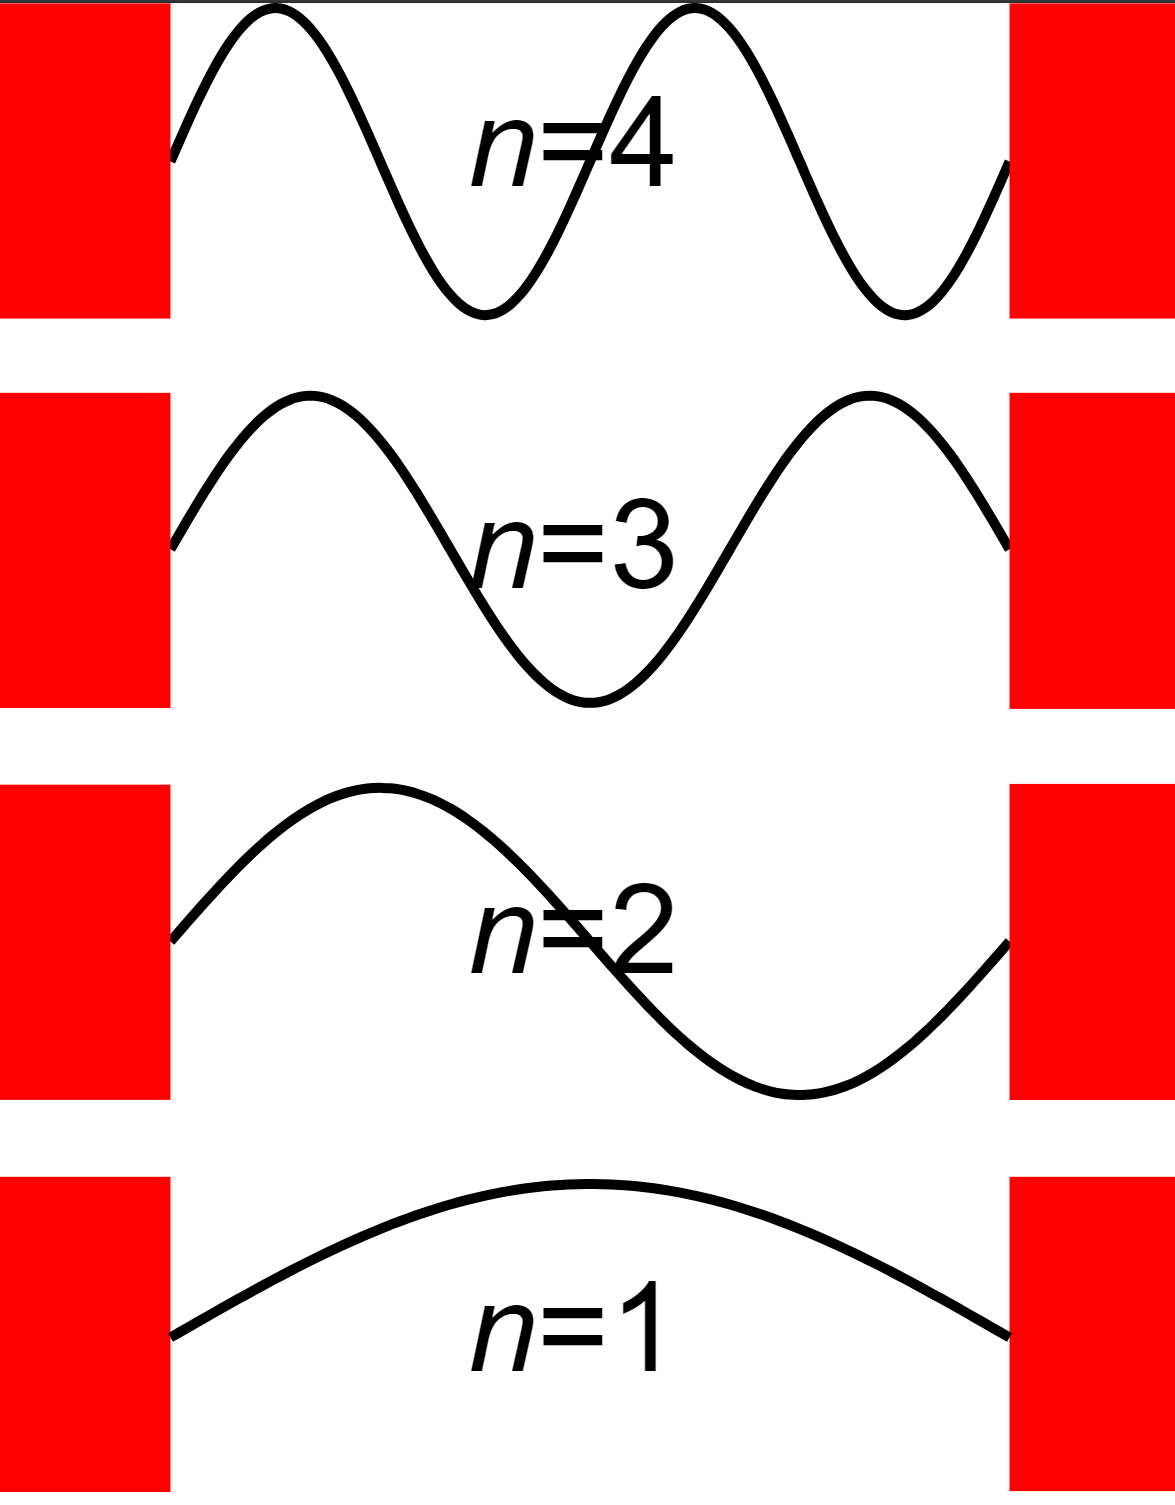
\includegraphics[width=.4\linewidth]{data/kasten.png}}
  \label{fig:kasten}
\end{figure}

%\begin{figure}
%  \centering
%  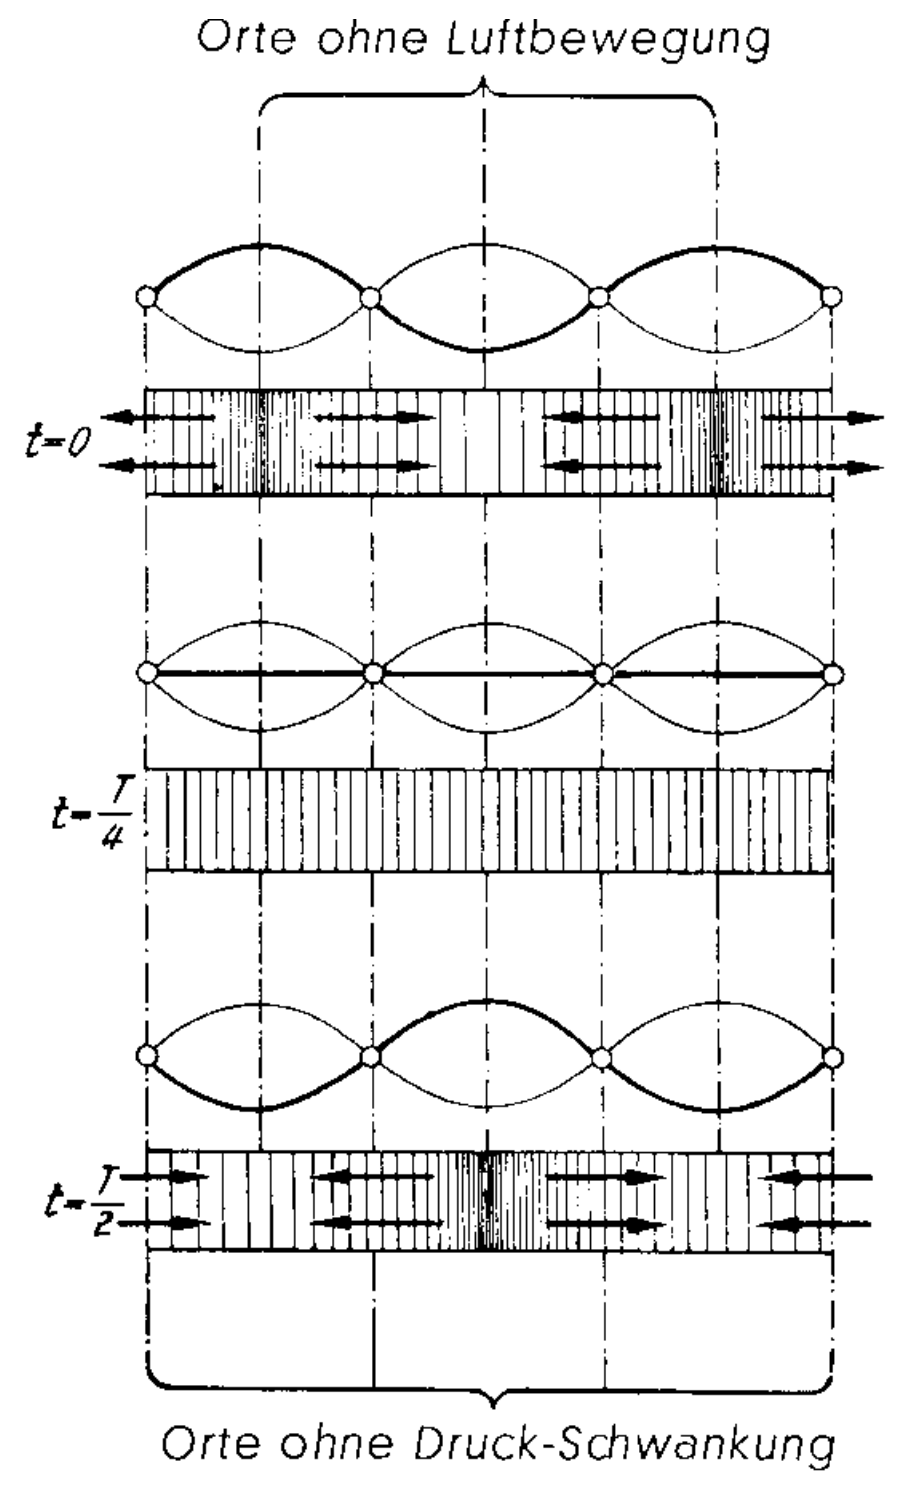
\includegraphics[width=\textwidth]{data/stehendeWelle.png}
%  \caption{Skizze der Luftbewegung und der Druckschwankung bei einer stehenden Welle \cite{stehendeWelle}.}
%  \label{fig:stehendeWelle}
%\end{figure}

\subsubsection{Teilchen im Kasten}
\label{subsubsec:kasten}
In der Quantenmechanik wird ein Teilchen der Masse $m$ vollständig durch eine orts- und zeitabhängige Wellenfunktion $\psi$ beschrieben. In der nichtrelativistischen Quantenmechanik ist die Bestimmungsgleichung für $\psi$ die zeitabhängige Schrödingergleichung in der Form
\begin{equation}
  i \hbar \frac{\partial \psi(\vec{r},t)}{\partial t} = H \psi(\vec{r},t) = \left(- \frac{\hbar^2}{2 m} \Laplace + V(\vec{r})\right) \psi(\vec{r},t)\,.
  \label{eqn:schroedingerZeitabhaengig}
\end{equation}
Dabei wurde explizit die Ortsdarstellung gewählt. Es bezeichnet $\hbar$ das reduzierte Plancksche Wirkungsquantum und $V$ ein zeitunabhängiges Potenzial. Der hermitesche Hamiltonoperator $H$ verfügt über Energieeigenwerte. Diese werden nach harmonischer Zeitabseperation $\psi(\vec{r},t) = \exp(-i E t / \hbar) \phi(\vec{r})$ in der zeitunabhängigen Schrödingergleichung
\begin{equation}
  E \phi(\vec{r}) = H \phi(\vec{r})
  \label{eqn:schroedingerZeitunabhaengig}
\end{equation}
sichtbar. Gefordert wird außerdem, dass der Zustand normiert sein muss, was im Falle der Ortsdarstellung durch die $L^2$-Norm realisiert wird: $\lvert\lvert \psi \rvert\rvert_{L^2} = 1\,.$ Observabel ist die Wellenfunktion $\psi$ selbst nicht. Stattdessen ist $\lvert \psi \rvert ^2$ die Aufenthaltswahrscheinlichkeitsdichte für das Teilchen. Dieser Zusammenhang verdeutlicht, dass die Quantenmechanik im Gegensatz zur klassischen Physik nichtdeterministisch ist. In ihrem System können für Messwerte nur Wahrscheinlichkeitsaussagen getroffen werden.
\\\\
Das Teilchen im Kasten (auch Teilchen im unendlich hohen Potenzialtopf genannt) ist ein klassisches einführendes Beispiel aus der Quantenmechanik. Der Kasten erstrecke sich (eindimensional) von 0 bis $L$, sodass sich das Teilchen dort frei bewegen kann. Dies entspricht einem Potenzial von $V \equiv 0$. Dort gilt also die zeitunabhängige Schrödingergleichung in der Form
\begin{equation}
  E \phi(x) = - \frac{\hbar^2}{2 m}  \frac{\partial^2 \phi(x)} {\partial x^2} \,.
  \label{eqn:schroedingerKasten}
\end{equation}
An den Wänden soll das Potenzial auf einen unendlich hohen Wert ansteigen, was so gedeutet werden kann, dass das Teilchen sich in dem Bereich außerhalb des Kastens nicht aufhalten kann.\\
Unter Beachtung der Normierung sind die Lösungen
\begin{equation}
  \psi_n(x,t)_ = \sqrt{\frac{2}{L}} \sin\left(\frac{n \pi x}{L}\right) \exp(-i E t / \hbar)\,.
  \label{eqn:kastenLoesung}
\end{equation}
Die ersten Wellenfunktion sind in Abbildung \ref{fig:kasten} dargestellt.

%\begin{figure}
%  \centering
%  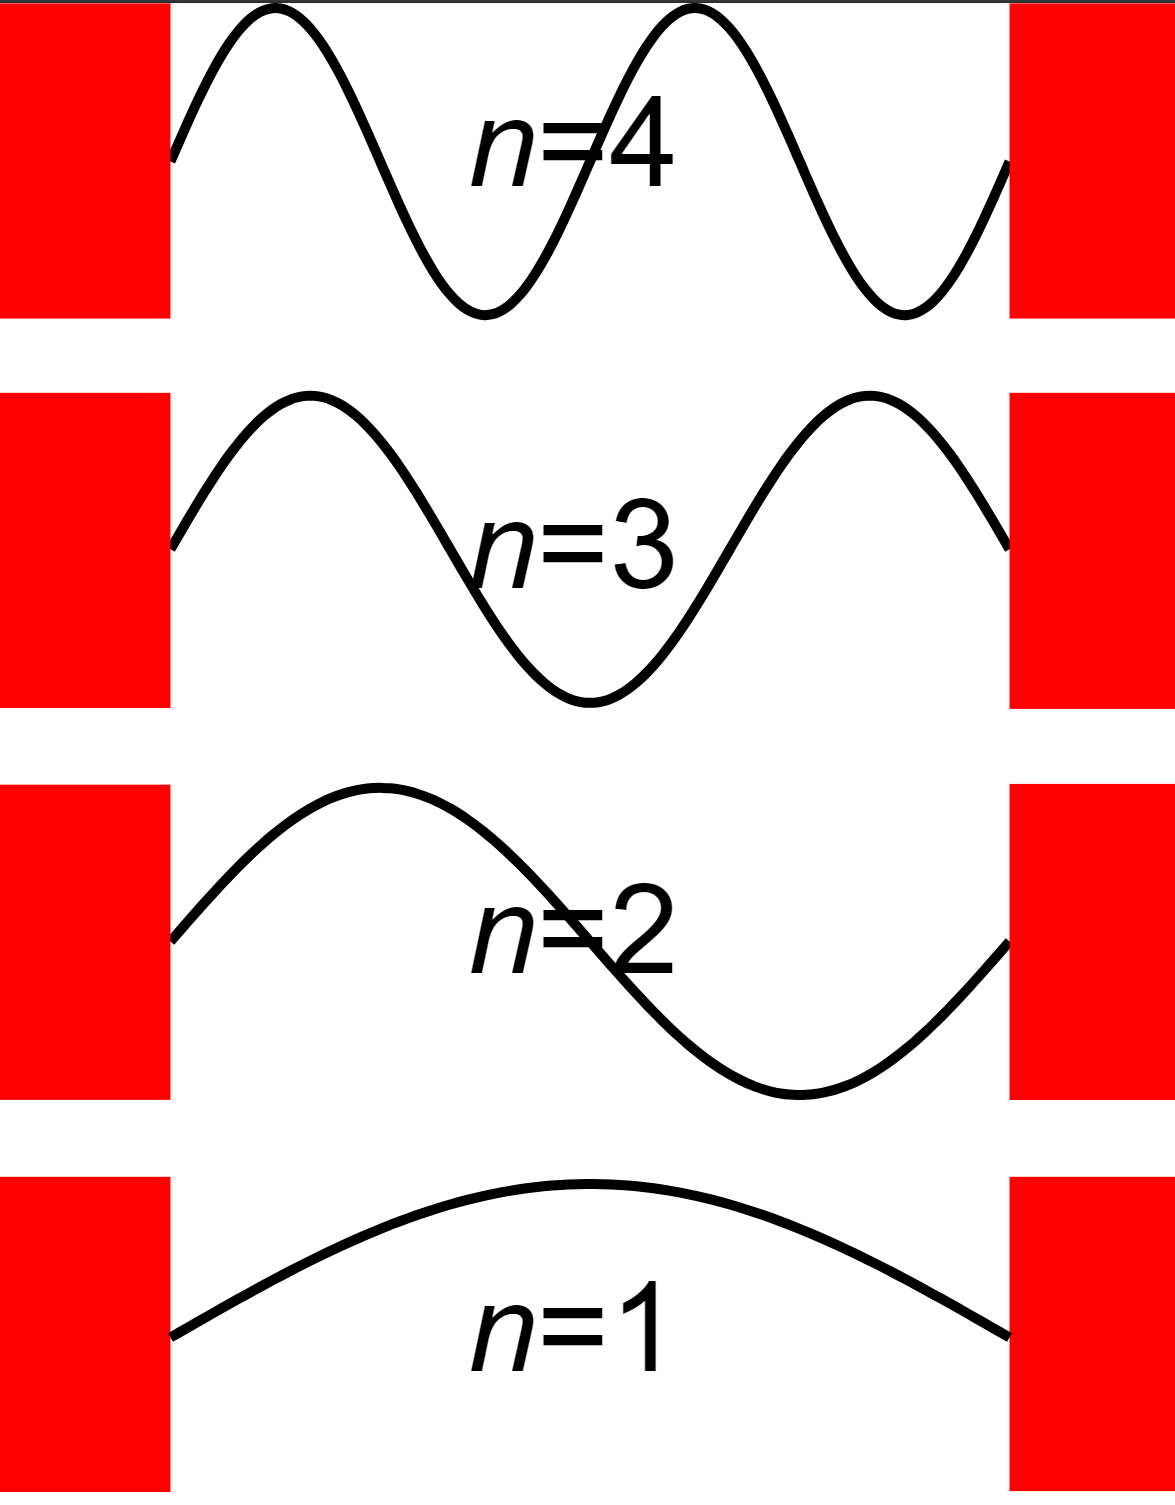
\includegraphics[width=\textwidth]{data/kasten.png}
%  \caption{Schematische Darstellung der ersten vier Wellenfunktionen im unendlich hohen Potenzialtopf \cite{kasten}.}
%  \label{fig:kasten}
%\end{figure}

Die Energieeigenwerte, also das Spektrum von H, lassen sich durch die Energiedispersionsrelation des freien Teilchens $E = \frac{\hbar^2 k^2}{2m}$ mit der Wellenzahl $k = 2 \pi / \lambda$ zu
\begin{equation}
  E_n = \frac{\hbar^2 \pi^2}{2 m L^2} n^2
  \label{eqn:kastenEnergien}
\end{equation}
bestimmen.

\subsubsection{Gemeinsamkeiten und Unterschiede der eindimensionalen Probleme}
Es ist ersichtlich, dass die Lösung für den Druck $p$ und die Wellenfunktion $\psi$ im Grunde mathematisch äquivalent sind. Die Wellenfunktion ist zwar komplex, jedoch beschreiben beide Funktionen stehende Wellen. Außerdem erfolgt in beiden Fällen die gleiche Diskretisierung bzw. Quantisierung der bestimmenden Größen (Eigenfrequenzen und Eigenenergien).\\
Diese Gemeinsamkeiten betreffen wichtige Charakteristika der Systeme und erlauben deswegen, eine Analogie zwischen ihnen zu sehen. Dennoch ergeben sich auch große Unterschiede, die sowohl bei der Berechnung als auch bei der Interpretation der Ergebnisse zu beachten sind:
\begin{itemize}
  \item Die Bestimmungsgleichungen unterscheiden sich in der Ordnung der zeitlichen Ableitung. Während die Wellengleichung zweiter Ordnung in der Zeit ist, sorgt bei der Schrödingergleichung die erste Ableitung multipliziert mit der imaginären Einheit für die harmonische Zeitabhängigkeit.
  \item Wie bereits erwähnt ist $\psi$ nicht direkt observabel, nur mit dem Betragsquadrat lassen sich statistische Aussagen treffen. Dagegen ist der Druck $p$ klassisch observabel.
  \item Die Randbedingungen unterscheiden sich. Während die Wellenfunktion an den Rändern des Kastens verschwinden muss, muss die stehende Druckwelle dort Bäuche aufweisen. Dies ist auch an den Abbildungen \ref{fig:stehendeWelle} und \ref{fig:kasten} ersichtlich. Dort haben Druckschwankung und Wellenfunktion gleiche Randbedingungen, sodass Druck (als Integral der Druckschwankung) und Wellenfunktion andere Randbedingungen haben müssen.
  \item Die Dispersionsrelationen für die beiden Regime der Physik unterscheiden sich grundlegend. In der klassischen Physik hängen Frequenz und Wellenzahl linear miteinander zusammen, während die Proportionalität in der Quantenmechanik quadratisch ist.
\end{itemize}

\subsection{Dreidimensionale Systeme}
\label{subsec:dreidimsyst}

\subsubsection{Theorie des Wasserstoffatoms}
\label{subsubsec:hatom}
Das Wasserstoffatom besteht aus einem zentralen Proton mit Ladung $+e$ und einem Hüllenelektron mit Ladung $-e$. Im Folgenden wird die Masse des Protons als unendlich im Vergleich zum Elektron genähert, sodass das Proton stationär ist. Es wird angenommen, dass beide Teilchen nur über die elektromagnetische Wechselwirkung interagieren. Die Problemstellung besteht also aus der Lösung der Schrödingergleichung mit dem radialsymmetrischen Coloumb-Potenzial
\begin{equation}
  V(r) = - \frac{1}{4 \pi \epsilon_0}{e^2}{r}\,.
  \label{eqn:coloumb}
\end{equation}
Um die Symmetrie des Problems zu berücksichtigen, werden Kugelkoordinaten gewählt. Der Laplace-Operator in der Schrödingergleichung hat in diesen Koordinaten einen radialen und einen Winkelteil:
\begin{equation}
  \Laplace = \Laplace_r + \frac{1}{r^2} \Laplace_{\theta, \varphi}\,.
  \label{eqn:laplaceWinkel}
\end{equation}
Somit erscheint ein Seperationsansatz sinnvoll. Es stellt sich heraus, dass die vollständige Lösung des Problems durch
\begin{equation}
  \psi_{nlm}(r,t) = R_{nl}(r) Y_{lm}(\theta, \varphi) \exp(-i E_n t / \hbar)
  \label{eqn:hatomloesung}
\end{equation}
gegeben ist. Dabei stellt $R_{nl}$ die Lösung des Radialteils dar, auf die nicht näher eingegangen werden sollen, weil sie für das theoretische Verständnis dieses Versuchs nicht weiter relevant sind. Der Winkelteil wird durch die sogenannten Kugelflächenfunktionen $Y_{lm}$ gelöst. Für sie gilt
\begin{equation}
  Y_{lm}(\theta,\varphi) = \frac{1}{\sqrt{2\pi}} N_{lm} P_{lm}(\cos\theta) \exp(im\varphi)\,.
  \label{eqn:kugelflaechenfunktionen}
\end{equation}
Dabei gilt für die Normierungskonstante
\begin{equation}
  N_{lm} = \sqrt{\frac{2l+1}{2} \frac{(l-m)!}{(l+m)!}}\,.
  \label{eqn:ylmnormierung}
\end{equation}
Die zugeordneten Legendrepolynome sind durch
\begin{equation}
  P_{lm}(x) = \frac{(-1)^m}{2^l l!} (1-x^2)^{\frac{m}{2}} \frac{\mathrm{d}^{l+m}}{\mathrm{d}x^{l+m}} (x^2-1)^l
  \label{eqn:zugeordneteLegendrepolynome}
\end{equation}
gegeben.\\
Die Wellenfunktionen werden Atomorbitale genannt. In Abbildung \ref{fig:kugelflaechenfunktionen} sind die Kugelflächenfunktionen, also der Winkelanteil, gezeigt. Diese tragen maßgeblich zur Form des Orbitals bei.

\begin{figure}
  \centering
  \includegraphics[width=\textwidth]{data/kugelschei.png}
  \caption{Darstellung des Betragsquadrats der ersten Kugelflächenfunktionen als Isoflächen \cite{kugelflaechenfunktionen}.}
  \label{fig:kugelflaechenfunktionen}
\end{figure}

Bestimmtes Merkmal der Lösungen ist ihre Quantisierung. Die Hauptquantenzahl $n$ ist Element der natürlichen Zahlen ohne null. Anschaulich gibt $n$ eine Art Bahn des Elektrons an, also in welchem Abstand sich das Elektron am wahrscheinlichsten aufhält. Die Drehimpulsquantenzahl $l$ geht von 0,1,... bis $n-1$ und beschreibt die räumliche Form des Orbitals. Die magnetische Quantenzahl $m$ kann ganzzahlige Werte von $-l$ bis $l$ annehmen und gibt die Projektion des Drehimpulses auf die $z$-Achse an.\\
Die Energieeigenwerte $E_n = -E_{\text{Ryd}}/n^2 \approx -\SI{13.6}{\electronvolt}/n^2$ hängen nur von $n$ ab. Sie sind somit in $l$ und $m$ entartet.
%Die $m$-Entartung kann durch das Anlegen eines schwachen magnetischen Feldes im Rahmen des Zeeman-Effektes aufgehoben werden. Dann wird die Rotationssymmetrie durch das Ausbilden einer Vorzugsrichtung des Magnetfeldes gebrochen. Die zu einem $l$ gehörenden Niveaus spalten in $(2m+1)$ sogenannte Zeeman-Niveaus auf.

\subsubsection{Der Kugelresonator}
\label{subsubsec:kugelresonator}
Wie beim Wasserstoffatom weist auch der kugelförmige Resonator eine radiale Symmetrie auf. Deswegen werden Kugelkoordinaten verwendet, sodass sich der Laplace-Operator in Gleichung \eqref{eqn:wellengleichung} wie in Gleichung \eqref{eqn:laplaceWinkel} in Radial- und Winkelanteil aufspaltet. Es ist einsichtig, dass der Winkelanteil der Lösung von $p(\vec{r}, t) = p(r,\theta,\varphi,t)$ gleich dem des Wasserstoffatoms sein muss; erneut ergeben sich Kugelflächenfunktionen. Die Radialanteile sind nicht gleich, da es sich bei dem Kugelresonator um ein freies Problem handelt. In der Sprache der Quantenmechanik entspricht das dem Fehlen eines Potenzialterms, klassisch bedeutet das, dass die Wellengleichung homogen ist.\\
Es ergibt sich, dass die Quantenzahlen $n'$, $l$ und $m$ zur Beschreibung der Moden des Resonators geeignet sind, wobei $n'$ in Ähnlichkeit zu $n$ eine Art radiale Quantenzahl darstellt. Eine $l$-Entartung liegt hier nicht vor. Die Entartung in $m$ bleibt als Einzige noch bestehen. %Es sei darauf hingewiesen, dass sich durch die Gegenüberstellung von Lautsprecher und Mikrophon Zylindersymmetrie ausbildet, wodurch sich in dieser Aufstellung größtenteils nur $m=0$-Zustände anregen lassen.
Aufgrund der Radialsymmetrie der Anordnung lassen sich größtenteils nur $m=0$-Zustände anregen. Ein Anbringen von sogenannten Zwischenringen an dem Kugelresonator kann dazu dienen, diese Symmetrie zu brechen und die Anregung von $m=\pm1$-Zuständen zu erlauben. Das quantenmechanische Analogon dazu ist der Zeeman-Effekt: Durch das Anlegen eines Magnetfeldes ergibt sich eine Vorzugsrichtung. Die Entartung der Zustände, die sich in der Quantenzahl $m$ unterscheiden, wird aufgehoben und ihre Energien unterscheiden sich.
